\documentclass{standalone}
\usepackage{tikz}
\usetikzlibrary{patterns, positioning}
\usepackage[sfdefault]{ClearSans} %% option 'sfdefault' activates Clear Sans as the default text font
\usepackage[T1]{fontenc}

\begin{document}
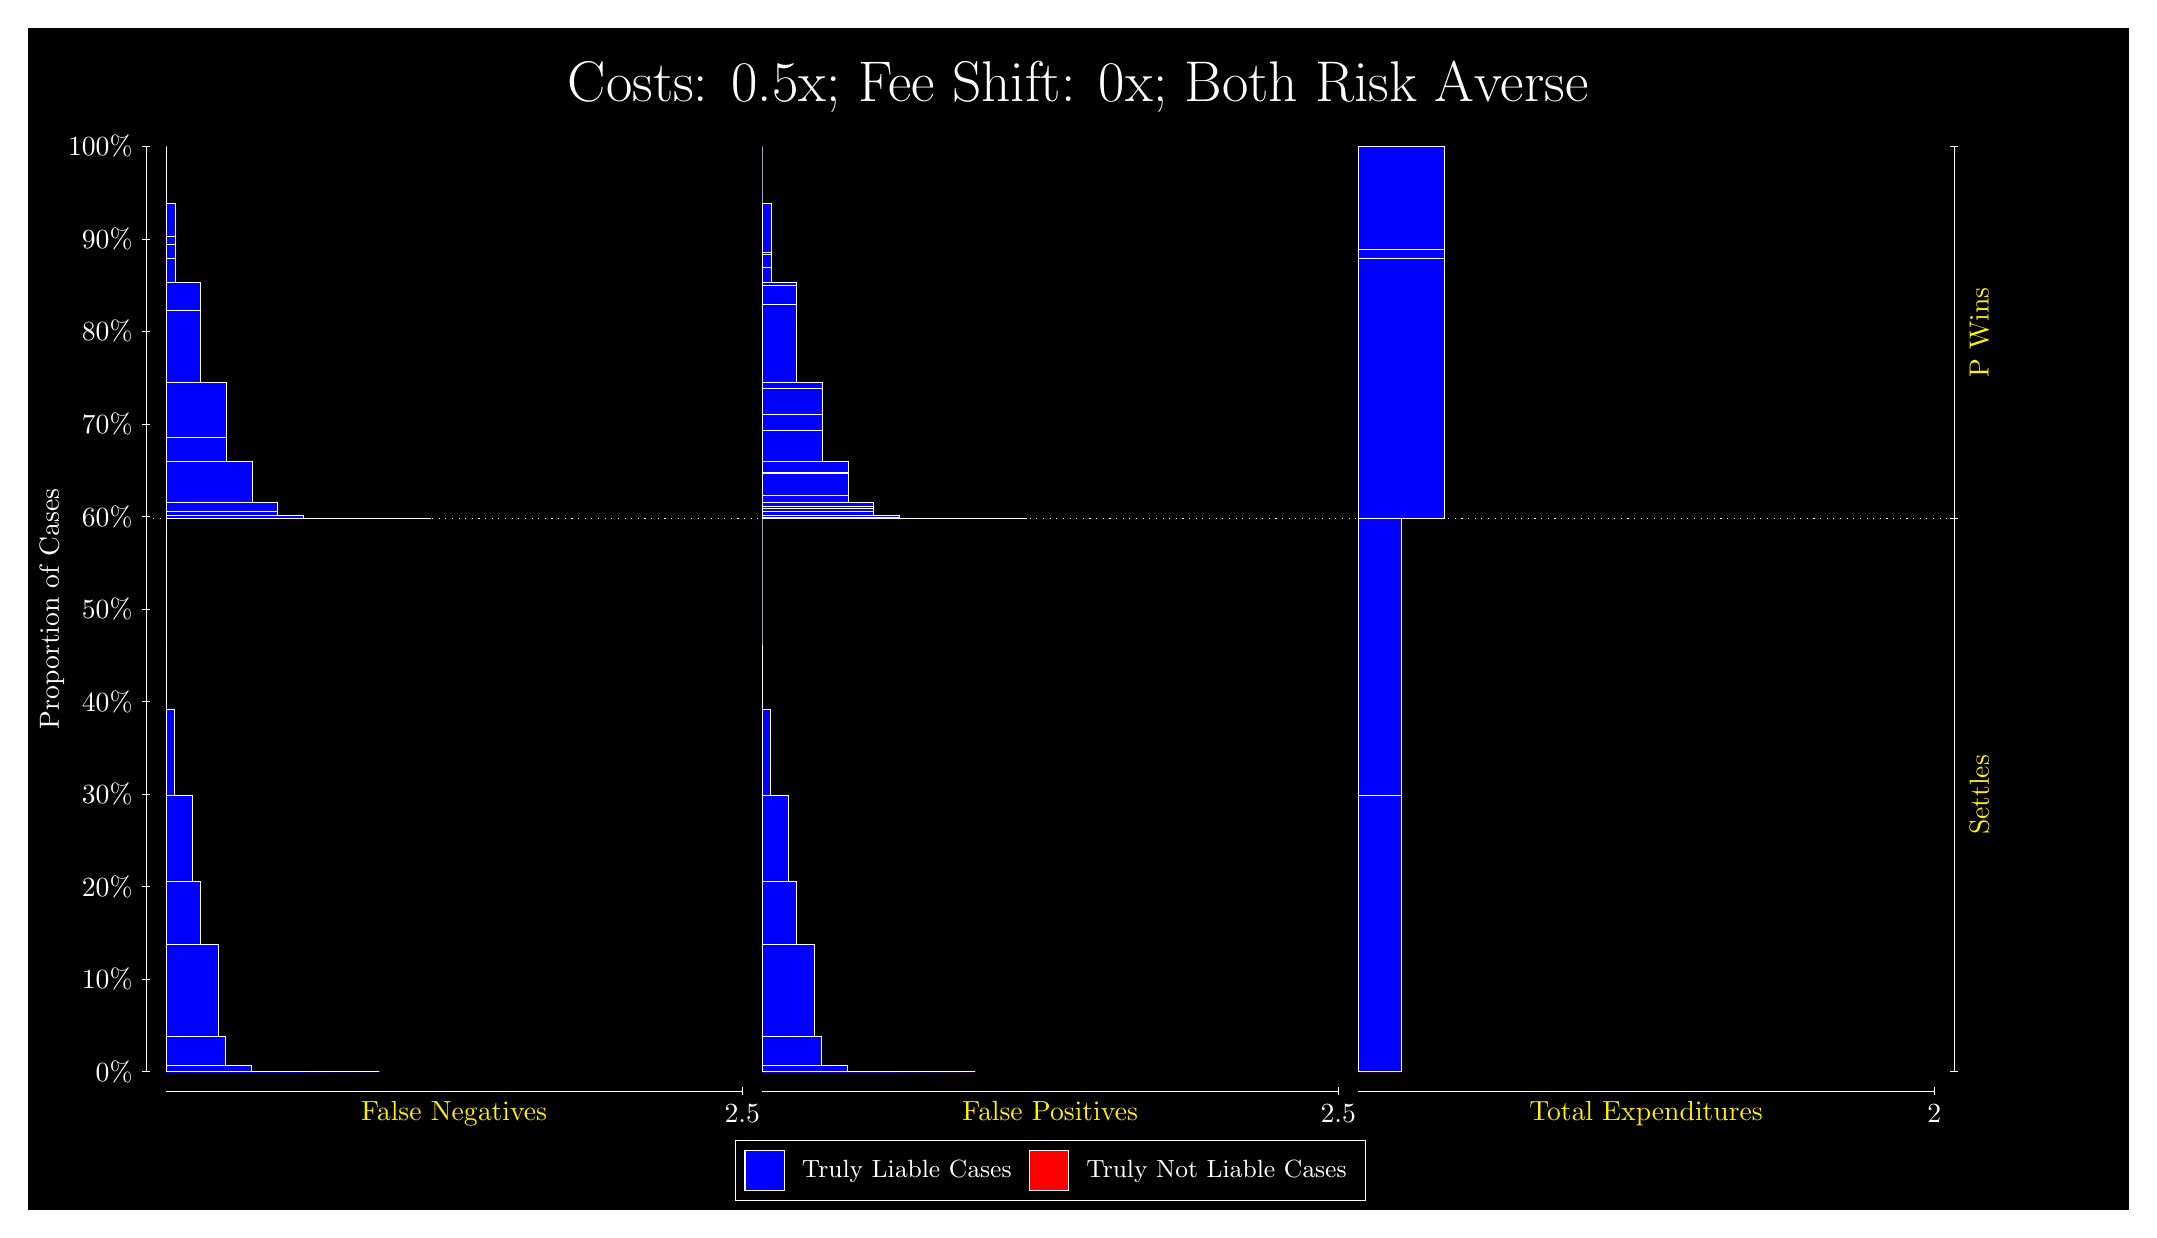
\begin{tikzpicture}
\draw[fill=black] (0,0) rectangle (26.667,15);
\draw[text=white] (0,13.5) rectangle (26.667,15) node[midway] {\huge Costs: 0.5x; Fee Shift: 0x; Both Risk Averse};
\draw[white, very thin] (1.5,1.75) -- (1.5,13.5);
\node[rotate=90, text=white, anchor=center] at (0.3, 7.625) {Proportion of Cases};
\draw[white, very thin] (1.45,1.75) -- (1.55,1.75);
\node[text=white, anchor=east] at (1.45, 1.75) {0\%};
\draw[white, very thin] (1.45,2.925) -- (1.55,2.925);
\node[text=white, anchor=east] at (1.45, 2.925) {10\%};
\draw[white, very thin] (1.45,4.1) -- (1.55,4.1);
\node[text=white, anchor=east] at (1.45, 4.1) {20\%};
\draw[white, very thin] (1.45,5.275) -- (1.55,5.275);
\node[text=white, anchor=east] at (1.45, 5.275) {30\%};
\draw[white, very thin] (1.45,6.45) -- (1.55,6.45);
\node[text=white, anchor=east] at (1.45, 6.45) {40\%};
\draw[white, very thin] (1.45,7.625) -- (1.55,7.625);
\node[text=white, anchor=east] at (1.45, 7.625) {50\%};
\draw[white, very thin] (1.45,8.8) -- (1.55,8.8);
\node[text=white, anchor=east] at (1.45, 8.8) {60\%};
\draw[white, very thin] (1.45,9.975) -- (1.55,9.975);
\node[text=white, anchor=east] at (1.45, 9.975) {70\%};
\draw[white, very thin] (1.45,11.15) -- (1.55,11.15);
\node[text=white, anchor=east] at (1.45, 11.15) {80\%};
\draw[white, very thin] (1.45,12.325) -- (1.55,12.325);
\node[text=white, anchor=east] at (1.45, 12.325) {90\%};
\draw[white, very thin] (1.45,13.5) -- (1.55,13.5);
\node[text=white, anchor=east] at (1.45, 13.5) {100\%};

\draw[white, very thin] (24.457,1.75) -- (24.457,13.5);
\draw[white, very thin] (24.407,1.75) -- (24.507,1.75);
\node[anchor=west] at (24.407, 1.75) {};
\draw[white, very thin] (24.407,8.7768) -- (24.507,8.7768);
\node[anchor=west] at (24.407, 8.7768) {};
\draw[white, very thin] (24.407,13.5) -- (24.507,13.5);
\node[anchor=west] at (24.407, 13.5) {};

\draw[white, very thin, fill=blue] (1.75,1.75) rectangle (4.458,1.75);
\draw[white, very thin, fill=blue] (1.75,1.75) rectangle (4.1327,1.75);
\draw[white, very thin, fill=blue] (1.75,1.75) rectangle (3.8074,1.75);
\draw[white, very thin, fill=blue] (1.75,1.75) rectangle (3.4821,1.7502);
\draw[white, very thin, fill=blue] (1.75,1.7502) rectangle (3.4333,1.7502);
\draw[white, very thin, fill=blue] (1.75,1.7502) rectangle (3.1568,1.757);
\draw[white, very thin, fill=blue] (1.75,1.757) rectangle (3.1081,1.757);
\draw[white, very thin, fill=blue] (1.75,1.757) rectangle (2.8316,1.835);
\draw[white, very thin, fill=blue] (1.75,1.835) rectangle (2.7828,1.835);
\draw[white, very thin, fill=blue] (1.75,1.835) rectangle (2.5063,2.1973);
\draw[white, very thin, fill=blue] (1.75,2.1973) rectangle (2.4575,2.1973);
\draw[white, very thin, fill=blue] (1.75,2.1973) rectangle (2.4087,3.3618);
\draw[white, very thin, fill=blue] (1.75,3.3618) rectangle (2.181,4.172);
\draw[white, very thin, fill=blue] (1.75,4.172) rectangle (2.1322,4.1725);
\draw[white, very thin, fill=blue] (1.75,4.1725) rectangle (2.0834,5.2634);
\draw[white, very thin, fill=blue] (1.75,5.2634) rectangle (1.8557,6.3543);
\draw[white, very thin, fill=blue] (1.75,6.3543) rectangle (1.8069,6.3548);
\draw[white, very thin, fill=blue] (1.75,6.3548) rectangle (1.7581,7.165);
\draw[white, very thin, fill=red] (1.75,7.165) rectangle (1.75,7.165);
\draw[white, very thin, fill=blue] (1.75,7.165) rectangle (1.75,8.7768);
\draw[white, very thin, fill=blue] (1.75,8.7768) rectangle (5.1167,8.7768);
\draw[white, very thin, fill=blue] (1.75,8.7768) rectangle (4.7914,8.7768);
\draw[white, very thin, fill=blue] (1.75,8.7768) rectangle (4.7914,8.7768);
\draw[white, very thin, fill=blue] (1.75,8.7768) rectangle (4.4661,8.7768);
\draw[white, very thin, fill=blue] (1.75,8.7768) rectangle (4.4661,8.7768);
\draw[white, very thin, fill=blue] (1.75,8.7768) rectangle (4.1408,8.7769);
\draw[white, very thin, fill=blue] (1.75,8.7769) rectangle (3.8155,8.7788);
\draw[white, very thin, fill=blue] (1.75,8.7788) rectangle (3.8155,8.7799);
\draw[white, very thin, fill=blue] (1.75,8.7799) rectangle (3.4903,8.8095);
\draw[white, very thin, fill=blue] (1.75,8.8095) rectangle (3.165,8.8662);
\draw[white, very thin, fill=blue] (1.75,8.8662) rectangle (3.165,8.9737);
\draw[white, very thin, fill=blue] (1.75,8.9737) rectangle (2.8397,9.4955);
\draw[white, very thin, fill=blue] (1.75,9.4955) rectangle (2.5144,9.8098);
\draw[white, very thin, fill=blue] (1.75,9.8098) rectangle (2.5144,10.509);
\draw[white, very thin, fill=blue] (1.75,10.509) rectangle (2.1891,11.423);
\draw[white, very thin, fill=blue] (1.75,11.423) rectangle (2.1891,11.768);
\draw[white, very thin, fill=blue] (1.75,11.768) rectangle (1.8638,12.079);
\draw[white, very thin, fill=blue] (1.75,12.079) rectangle (1.8638,12.252);
\draw[white, very thin, fill=blue] (1.75,12.252) rectangle (1.8638,12.357);
\draw[white, very thin, fill=blue] (1.75,12.357) rectangle (1.8638,12.781);
\draw[white, very thin, fill=red] (1.75,12.781) rectangle (1.75,12.781);
\draw[white, very thin, fill=blue] (1.75,12.781) rectangle (1.75,13.5);
\draw[white, very thin, fill=red] (9.3189,1.75) rectangle (12.027,1.75);
\draw[white, very thin, fill=blue] (9.3189,1.75) rectangle (12.027,1.75);
\draw[white, very thin, fill=blue] (9.3189,1.75) rectangle (11.702,1.75);
\draw[white, very thin, fill=blue] (9.3189,1.75) rectangle (11.376,1.75);
\draw[white, very thin, fill=blue] (9.3189,1.75) rectangle (11.051,1.7502);
\draw[white, very thin, fill=red] (9.3189,1.7502) rectangle (11.002,1.7502);
\draw[white, very thin, fill=blue] (9.3189,1.7502) rectangle (11.002,1.7502);
\draw[white, very thin, fill=blue] (9.3189,1.7502) rectangle (10.726,1.757);
\draw[white, very thin, fill=blue] (9.3189,1.757) rectangle (10.677,1.757);
\draw[white, very thin, fill=blue] (9.3189,1.757) rectangle (10.4,1.835);
\draw[white, very thin, fill=blue] (9.3189,1.835) rectangle (10.352,1.835);
\draw[white, very thin, fill=blue] (9.3189,1.835) rectangle (10.075,2.1973);
\draw[white, very thin, fill=blue] (9.3189,2.1973) rectangle (10.026,2.1973);
\draw[white, very thin, fill=red] (9.3189,2.1973) rectangle (9.9776,2.1973);
\draw[white, very thin, fill=blue] (9.3189,2.1973) rectangle (9.9776,3.3618);
\draw[white, very thin, fill=blue] (9.3189,3.3618) rectangle (9.7499,4.172);
\draw[white, very thin, fill=blue] (9.3189,4.172) rectangle (9.7011,4.1725);
\draw[white, very thin, fill=blue] (9.3189,4.1725) rectangle (9.6523,5.2634);
\draw[white, very thin, fill=blue] (9.3189,5.2634) rectangle (9.4246,6.3543);
\draw[white, very thin, fill=blue] (9.3189,6.3543) rectangle (9.3758,6.3548);
\draw[white, very thin, fill=blue] (9.3189,6.3548) rectangle (9.327,7.165);
\draw[white, very thin, fill=blue] (9.3189,7.165) rectangle (9.3189,8.7768);
\draw[white, very thin, fill=red] (9.3189,8.7768) rectangle (12.686,8.7768);
\draw[white, very thin, fill=blue] (9.3189,8.7768) rectangle (12.686,8.7768);
\draw[white, very thin, fill=red] (9.3189,8.7768) rectangle (12.36,8.7768);
\draw[white, very thin, fill=blue] (9.3189,8.7768) rectangle (12.36,8.7768);
\draw[white, very thin, fill=red] (9.3189,8.7768) rectangle (12.035,8.7768);
\draw[white, very thin, fill=blue] (9.3189,8.7768) rectangle (12.035,8.7768);
\draw[white, very thin, fill=blue] (9.3189,8.7768) rectangle (12.035,8.7768);
\draw[white, very thin, fill=blue] (9.3189,8.7768) rectangle (12.035,8.7768);
\draw[white, very thin, fill=red] (9.3189,8.7768) rectangle (11.71,8.7768);
\draw[white, very thin, fill=blue] (9.3189,8.7768) rectangle (11.71,8.7769);
\draw[white, very thin, fill=blue] (9.3189,8.7769) rectangle (11.71,8.7769);
\draw[white, very thin, fill=red] (9.3189,8.7769) rectangle (11.384,8.7769);
\draw[white, very thin, fill=blue] (9.3189,8.7769) rectangle (11.384,8.7774);
\draw[white, very thin, fill=blue] (9.3189,8.7774) rectangle (11.384,8.7799);
\draw[white, very thin, fill=blue] (9.3189,8.7799) rectangle (11.059,8.7877);
\draw[white, very thin, fill=red] (9.3189,8.7877) rectangle (11.059,8.7877);
\draw[white, very thin, fill=blue] (9.3189,8.7877) rectangle (11.059,8.7911);
\draw[white, very thin, fill=blue] (9.3189,8.7911) rectangle (11.059,8.8095);
\draw[white, very thin, fill=blue] (9.3189,8.8095) rectangle (10.734,8.8655);
\draw[white, very thin, fill=blue] (9.3189,8.8655) rectangle (10.734,8.9005);
\draw[white, very thin, fill=red] (9.3189,8.9005) rectangle (10.734,8.9005);
\draw[white, very thin, fill=blue] (9.3189,8.9005) rectangle (10.734,8.9323);
\draw[white, very thin, fill=blue] (9.3189,8.9323) rectangle (10.734,8.9737);
\draw[white, very thin, fill=blue] (9.3189,8.9737) rectangle (10.409,9.0647);
\draw[white, very thin, fill=red] (9.3189,9.0647) rectangle (10.409,9.0647);
\draw[white, very thin, fill=blue] (9.3189,9.0647) rectangle (10.409,9.351);
\draw[white, very thin, fill=blue] (9.3189,9.351) rectangle (10.409,9.3621);
\draw[white, very thin, fill=blue] (9.3189,9.3621) rectangle (10.409,9.4955);
\draw[white, very thin, fill=blue] (9.3189,9.4955) rectangle (10.083,9.8985);
\draw[white, very thin, fill=blue] (9.3189,9.8985) rectangle (10.083,10.093);
\draw[white, very thin, fill=red] (9.3189,10.093) rectangle (10.083,10.093);
\draw[white, very thin, fill=blue] (9.3189,10.093) rectangle (10.083,10.428);
\draw[white, very thin, fill=blue] (9.3189,10.428) rectangle (10.083,10.509);
\draw[white, very thin, fill=blue] (9.3189,10.509) rectangle (9.758,11.493);
\draw[white, very thin, fill=red] (9.3189,11.493) rectangle (9.758,11.493);
\draw[white, very thin, fill=blue] (9.3189,11.493) rectangle (9.758,11.497);
\draw[white, very thin, fill=blue] (9.3189,11.497) rectangle (9.758,11.738);
\draw[white, very thin, fill=blue] (9.3189,11.738) rectangle (9.758,11.768);
\draw[white, very thin, fill=blue] (9.3189,11.768) rectangle (9.4327,11.962);
\draw[white, very thin, fill=blue] (9.3189,11.962) rectangle (9.4327,12.135);
\draw[white, very thin, fill=blue] (9.3189,12.135) rectangle (9.4327,12.156);
\draw[white, very thin, fill=blue] (9.3189,12.156) rectangle (9.4327,12.778);
\draw[white, very thin, fill=blue] (9.3189,12.778) rectangle (9.4327,12.781);
\draw[white, very thin, fill=blue] (9.3189,12.781) rectangle (9.3189,13.5);
\draw[white, very thin, fill=red] (16.888,1.75) rectangle (17.437,1.75);
\draw[white, very thin, fill=blue] (16.888,1.75) rectangle (17.437,5.264);
\draw[white, very thin, fill=red] (16.888,5.264) rectangle (17.437,5.264);
\draw[white, very thin, fill=blue] (16.888,5.264) rectangle (17.437,8.7768);
\draw[white, very thin, fill=red] (16.888,8.7768) rectangle (17.986,8.7768);
\draw[white, very thin, fill=blue] (16.888,8.7768) rectangle (17.986,12.082);
\draw[white, very thin, fill=red] (16.888,12.082) rectangle (17.986,12.082);
\draw[white, very thin, fill=blue] (16.888,12.082) rectangle (17.986,12.192);
\draw[white, very thin, fill=red] (16.888,12.192) rectangle (17.986,12.192);
\draw[white, very thin, fill=blue] (16.888,12.192) rectangle (17.986,13.5);
\draw[white, dotted] (1.5,8.7768) -- (24.457,8.7768);
\draw[white, very thin] (1.75,1.5) -- (9.0689,1.5);
\node[text=yellow, anchor=north] at (5.4094, 1.5) {False Negatives};
\draw[white, very thin] (9.0689,1.45) -- (9.0689,1.55);
\node[text=white, anchor=north] at (9.0689, 1.45) {2.5};

\draw[white, very thin] (9.3189,1.5) -- (16.638,1.5);
\node[text=yellow, anchor=north] at (12.978, 1.5) {False Positives};
\draw[white, very thin] (16.638,1.45) -- (16.638,1.55);
\node[text=white, anchor=north] at (16.638, 1.45) {2.5};

\draw[white, very thin] (16.888,1.5) -- (24.207,1.5);
\node[text=yellow, anchor=north] at (20.547, 1.5) {Total Expenditures};
\draw[white, very thin] (24.207,1.45) -- (24.207,1.55);
\node[text=white, anchor=north] at (24.207, 1.45) {2};

\node[text=yellow, centered, rotate=90] at (24.777, 5.2634) {Settles};
\node[text=yellow, centered, rotate=90] at (24.777, 11.138) {P Wins};

\draw (12.978300999999998,1.5) node[draw=none] (baseCoordinate) {};
\begin{scope}[align=center]
        \matrix[scale=0.5, draw=white, below=0.5cm of baseCoordinate, nodes={draw}, column sep=0.1cm]{
            \node[rectangle, draw, minimum width=0.5cm, minimum height=0.5cm, fill=blue] {}; &
            \node[draw=none, font=\small, text=white] (B) {Truly Liable Cases}; &
            \node[rectangle, draw, minimum width=0.5cm, minimum height=0.5cm, fill=red] {}; &
            \node[draw=none, font=\small, text=white] (B) {Truly Not Liable Cases}; \\
            };
\end{scope}

\end{tikzpicture}
\end{document}